\documentclass[aspectratio=169,11pt]{beamer}

\usetheme{Madrid}
\setbeamertemplate{navigation symbols}{}
\setbeamertemplate{footline}[frame number]
\usepackage[T1]{fontenc}
\usepackage[utf8]{inputenc}
\usepackage{amsmath}
\usepackage{booktabs}
\usepackage{array}
\usepackage{xcolor}
\usepackage{tikz}
\usetikzlibrary{arrows.meta,positioning,shapes.geometric}
\usepackage{listings}
\usepackage{hyperref}

\definecolor{concordiablue}{RGB}{20,60,120}
\definecolor{softgray}{RGB}{245,247,250}
\definecolor{codegray}{RGB}{248,248,248}

\setbeamercolor{title}{fg=white,bg=concordiablue}
\setbeamercolor{frametitle}{fg=white,bg=concordiablue}
\setbeamercolor{block title}{fg=white,bg=concordiablue}
\setbeamercolor{block body}{bg=softgray,fg=black}

\lstdefinestyle{codestyle}{
  basicstyle=\ttfamily\scriptsize,
  backgroundcolor=\color{codegray},
  showstringspaces=false,
  breaklines=true,
  frame=single,
  columns=fullflexible
}

\title[SOEN 6011 D2 - F3]{Delivery 2: F3 - Hyperbolic Sine $\sinh(x)$}
\subtitle{From-scratch Python implementation with Tkinter GUI}
\author{Arvind Lakshmanan (40310757)}
\institute{SOEN 6011: Software Engineering Processes\\Concordia University}
\date{Summer 2026}

\begin{document}

\begin{frame}
\titlepage
\vspace{-0.3cm}
\begin{center}
\small Assigned function: \textbf{F3: $\sinh(x)$}
\end{center}
\end{frame}

\begin{frame}{D2 Roadmap}
\large
\begin{enumerate}
    \item Modify D1 implementation into a from-scratch version.
    \item Add a Tkinter graphical user interface.
    \item Handle exceptions with helpful messages.
    \item Prepare public version-control evidence.
    \item Update requirements based on the D2 implementation.
\end{enumerate}
\end{frame}

\begin{frame}{D1 to D2 Change}
\begin{columns}[T]
\begin{column}{0.48\textwidth}
\begin{block}{D1 implementation}
\begin{itemize}
    \item Textual interface.
    \item Used direct formula:
    \[
    \sinh(x)=\frac{e^x-e^{-x}}{2}
    \]
    \item Used \texttt{math.exp}.
\end{itemize}
\end{block}
\end{column}
\begin{column}{0.48\textwidth}
\begin{block}{D2 implementation}
\begin{itemize}
    \item Tkinter GUI.
    \item Uses Maclaurin series:
    \[
    \sinh(x)=x+\frac{x^3}{3!}+\frac{x^5}{5!}+\cdots
    \]
    \item No Python math-library function for calculation.
\end{itemize}
\end{block}
\end{column}
\end{columns}
\end{frame}

\begin{frame}{Problem 5: From-scratch Algorithm}
\centering
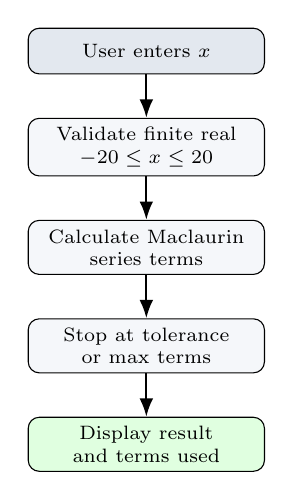
\begin{tikzpicture}[node distance=0.55cm, every node/.style={font=\scriptsize}, box/.style={draw,rounded corners,fill=softgray,align=center,minimum width=3.0cm,minimum height=0.58cm}]
\node[box, fill=concordiablue!12] (input) {User enters $x$};
\node[box, below=of input] (validate) {Validate finite real\\$-20 \leq x \leq 20$};
\node[box, below=of validate] (series) {Calculate Maclaurin\\series terms};
\node[box, below=of series] (stop) {Stop at tolerance\\or max terms};
\node[box, below=of stop, fill=green!12] (output) {Display result\\and terms used};
\draw[-Latex, thick] (input) -- (validate);
\draw[-Latex, thick] (validate) -- (series);
\draw[-Latex, thick] (series) -- (stop);
\draw[-Latex, thick] (stop) -- (output);
\end{tikzpicture}
\vspace{0.15cm}

\small The implementation separates validation, calculation, stopping logic, and output.
\end{frame}

\begin{frame}[fragile]{Problem 5: Series Recurrence}
\begin{lstlisting}[style=codestyle]
term_0 = x
sum = x

term_n = term_(n-1) * x^2 / ((2n) * (2n + 1))
sum = sum + term_n

stop when:
|term_n| <= tolerance * (1 + |sum|)
\end{lstlisting}
\vspace{0.2cm}
\begin{block}{Scratch implementation evidence}
The calculation avoids \texttt{math.sinh}, \texttt{math.exp}, \texttt{math.factorial}, NumPy, and SciPy.
\end{block}
\end{frame}

\begin{frame}{Problem 5: GUI and Exceptions}
\begin{columns}[T]
\begin{column}{0.48\textwidth}
\begin{block}{Tkinter GUI includes}
\begin{itemize}
    \item input box for $x$,
    \item Calculate button,
    \item Clear button,
    \item Exit button,
    \item result and status area.
\end{itemize}
\end{block}
\end{column}
\begin{column}{0.48\textwidth}
\begin{block}{Handled errors}
\begin{itemize}
    \item blank input,
    \item non-numeric input,
    \item NaN or infinity,
    \item out-of-range input,
    \item convergence failure.
\end{itemize}
\end{block}
\end{column}
\end{columns}
\end{frame}

% =========================================================
% SLIDE 1 — TKINTER APPLICATION INITIALISATION
% =========================================================

\begin{frame}[t]{Problem 5: Tkinter Application Initialisation}
\small

\begin{block}{Main GUI Class}
The \texttt{SinhCalculatorApp} class contains the graphical user
interface and connects the interface to the $\sinh(x)$ calculation.
\end{block}

\begin{description}

\item[\texttt{\_\_init\_\_(self, root)}]
Initialises the application and receives the main Tkinter window as
the \texttt{root} parameter.

\item[\texttt{root.title()}]
Sets the title displayed at the top of the application window.

\item[\texttt{root.geometry()}]
Defines the initial window size as $640 \times 420$ pixels.

\item[\texttt{root.minsize()}]
Prevents the user from resizing the window below
$560 \times 360$ pixels.

\item[\texttt{tk.StringVar()}]
Creates variables that automatically connect Python values to
Tkinter widgets.

\item[\texttt{self.input\_value}]
Stores the value entered by the user in the input field.

\item[\texttt{self.status\_value}]
Stores the status message displayed at the bottom of the GUI.

\item[\texttt{self.create\_widgets()}]
Calls the method responsible for creating and arranging all
interface components.

\end{description}

\begin{alertblock}{Purpose}
The initialisation method prepares the window, creates shared GUI
variables, and then constructs the complete user interface.
\end{alertblock}

\end{frame}


% =========================================================
% SLIDE 2 — TKINTER WIDGETS AND LAYOUT
% =========================================================

\begin{frame}[t]{Problem 5: Tkinter Widgets Used in the Application}
\scriptsize

\renewcommand{\arraystretch}{1.25}
\begin{tabular}{>{\bfseries}p{0.23\textwidth}p{0.68\textwidth}}

\texttt{ttk.Frame} &
Groups related widgets into sections such as the main area,
input area, and button area. \\

\texttt{ttk.Label} &
Displays the application title, instructions, input label,
result label, and status message. \\

\texttt{ttk.Entry} &
Provides the text field where the user enters the value of $x$.
It is connected to \texttt{self.input\_value}. \\

\texttt{ttk.Button} &
Creates the Calculate, Clear, and Exit buttons. Each button
calls a specific method through its \texttt{command} property. \\

\texttt{tk.Text} &
Displays the calculated result, number of terms used, algorithm
description, or error message. \\

\texttt{pack()} &
Places widgets inside their parent frames and controls their
position, spacing, and resizing behaviour. \\

\texttt{fill="x"} &
Allows a widget or frame to expand horizontally. \\

\texttt{fill="both"} &
Allows the result area to expand horizontally and vertically. \\

\texttt{expand=True} &
Uses the available extra space when the window is resized. \\

\texttt{padx} and \texttt{pady} &
Add horizontal and vertical spacing between interface components. \\

\end{tabular}
\end{frame}


% =========================================================
% SLIDE 3 — EVENTS, BUTTONS, AND RESULT DISPLAY
% =========================================================

\begin{frame}[t]{Problem 5: Tkinter Event Handling and GUI Functions}
\scriptsize

\begin{description}

\item[\texttt{input\_entry.focus()}]
Places the cursor inside the input field when the program starts,
allowing the user to type immediately.

\item[\texttt{input\_entry.bind("<Return>", self.calculate)}]
Connects the Enter key to the \texttt{calculate()} method. Therefore,
the user can calculate the result without clicking the button.

\item[\texttt{command=self.calculate}]
Calls the calculation method when the Calculate button is clicked.

\item[\texttt{command=self.clear}]
Calls the \texttt{clear()} method when the Clear button is clicked.

\item[\texttt{command=self.root.destroy}]
Closes the Tkinter window when the Exit button is clicked.

\item[\texttt{calculate(self, event=None)}]
Reads the input, validates it, calls the from-scratch
$\sinh(x)$ algorithm, and displays either the result or an error.

\item[\texttt{set\_result\_text(self, message)}]
Temporarily enables the result box, removes its previous content,
inserts the new message, and disables editing again.

\item[\texttt{clear(self)}]
Clears the input field, resets the result box, and restores the
initial status message.

\item[\texttt{status\_value.set()}]
Changes the status label after a successful calculation, invalid
input, convergence failure, or unexpected error.

\end{description}

\end{frame}


% =========================================================
% OPTIONAL SLIDE — PROGRAM EXECUTION
% =========================================================

\begin{frame}[t]{Problem 5: Starting the Tkinter Application}
\small

\begin{block}{The \texttt{main()} Function}
The \texttt{main()} function creates the root window, creates an
instance of the GUI class, and starts Tkinter's event loop.
\end{block}

\begin{enumerate}

\item
\texttt{root = tk.Tk()}

Creates the main application window.

\vspace{0.25cm}

\item
\texttt{app = SinhCalculatorApp(root)}

Creates the calculator interface inside the root window.

\vspace{0.25cm}

\item
\texttt{root.mainloop()}

Starts Tkinter's event loop and keeps the application running while
waiting for user actions.

\end{enumerate}
\end{frame}

\begin{frame}{Problem 5: Manual Validation Evidence}
\centering
\begin{tabular}{r r l}
\toprule
\textbf{Input} & \textbf{Approximate result} & \textbf{Case} \\
\midrule
0 & 0 & zero \\
1 & 1.1752011936438 & positive \\
-1 & -1.1752011936438 & negative \\
3 & 10.0178749274099 & larger input \\
20 & 242582597.704895 & upper boundary \\
\bottomrule
\end{tabular}
\end{frame}

% =========================================================
% SLIDE 1 — GIT AND GITHUB COMMANDS
% =========================================================

\begin{frame}[t]{Problem 6: Git and GitHub Commands Used}
\scriptsize

\begin{block}{Repository}
\centering
\url{https://github.com/arvind-mocha/SOFTWARE_ENGINEERING_PROCESSESUMMER_2026}
\end{block}

\begin{description}

\item[\texttt{git init -b main}]
Initialised the project folder as a Git repository with
\texttt{main} as the default branch.

\item[\texttt{git status}]
Displayed modified, untracked, and staged files before each commit.

\item[\texttt{git add .}]
Added all current project changes to Git's staging area.

\item[\texttt{git commit -m "message"}]
Created a permanent project revision with a descriptive commit message.

\item[\texttt{git remote add origin URL}]
Connected the local Git repository to the public GitHub repository.

\item[\texttt{git remote -v}]
Verified that the correct GitHub repository was configured as
\texttt{origin}.

\item[\texttt{git push -u origin main}]
Uploaded the initial commit history and linked the local
\texttt{main} branch to GitHub.

\item[\texttt{git push origin main}]
Uploaded subsequent local commits to the public GitHub repository.

\item[\texttt{git log --oneline}]
Displayed a concise list of commit identifiers and commit messages.

\end{description}

\end{frame}


\begin{frame}{Problem 6: Version Control Evidence}
\begin{block}{High-quality commits}
\begin{itemize}
    \item \texttt{Add validation for empty and non-numeric input}
    \item \texttt{Added real number support feature}
    \item \texttt{Added sinh calculation logic from scratch}
    \item \texttt{Added GUI using tkinter}
    \item \texttt{Pending features added to the GUI}
\end{itemize}
\end{block}
\end{frame}

% =========================================================
% SLIDE 2 — COMMIT MESSAGES AND EXPLANATIONS
% =========================================================

\begin{frame}[t]{Problem 6: Commit History}
\scriptsize

\begin{enumerate}

\item
\texttt{docs: add D2 README with setup and run instructions}

\textbf{Explanation:}
Added the project description, requirements, supported input range,
repository structure, and instructions for running the application.

\vspace{0.15cm}

\item
\texttt{feat: implement from-scratch Maclaurin series for sinh}

\textbf{Explanation:}
Added the core numerical algorithm for calculating $\sinh(x)$ without
using prohibited Python mathematical-library functions.

\vspace{0.15cm}

\item
\texttt{feat: add Tkinter GUI with input validation and helpful errors}

\textbf{Explanation:}
Added the graphical interface, user-input controls, validation,
exception handling, and understandable error messages.

\vspace{0.15cm}

\item
\texttt{refactor: separate parsing, calculation, and GUI responsibilities}

\textbf{Explanation:}
Separated input processing, mathematical calculation, and interface
logic to improve readability and maintainability.

\vspace{0.15cm}

\item
\texttt{docs: update D2 requirements and traceability}

\textbf{Explanation:}
Documented the updated requirements and connected them to the
from-scratch algorithm, GUI, exception handling, and repository changes.

\end{enumerate}
\end{frame}


\begin{frame}{Problem 7: Updated Requirements}
\small
\begin{tabular}{p{0.18\textwidth}p{0.64\textwidth}p{0.1\textwidth}}
\toprule
\textbf{ID} & \textbf{Requirement} & \textbf{Priority} \\
\midrule
REQ-F3-D2-01 & The system shall provide a Tkinter graphical user interface. & High \\
REQ-F3-D2-03 & The system shall support inputs in $[-20,20]$. & High \\
REQ-F3-D2-04 & The system shall calculate $\sinh(x)$ using a from-scratch Maclaurin series. & High \\
REQ-F3-D2-05 & The system shall not use prohibited math-library functions for calculation. & High \\
REQ-F3-D2-07 & The system shall provide helpful errors for invalid inputs. & High \\
REQ-F3-D2-12 & The source code shall be placed in a public distributed version control system with a README. & High \\
\bottomrule
\end{tabular}
\end{frame}

\begin{frame}{GAI Use: CASTROFF Summary}
\small
\begin{tabular}{p{0.18\textwidth}p{0.37\textwidth}p{0.36\textwidth}}
\toprule
\textbf{Problem} & \textbf{Prompt type} & \textbf{How output was used} \\
\midrule
P5 & Implementation-generation prompt with constraints & Helped structure scratch algorithm, GUI, and exceptions. \\
P6 & Documentation and version-control planning prompt & Helped prepare README and commit-message examples. \\
P7 & Requirements-revision prompt & Helped update requirements and trace D1 changes to D2. \\
\bottomrule
\end{tabular}
\end{frame}



\begin{frame}{Conclusion}
\large
For D2, the F3 calculator was modified from a D1 textual implementation into a Tkinter GUI application. The calculation now uses a from-scratch Maclaurin series, includes exception handling with helpful messages, has repository documentation, and includes an updated list of requirements aligned with the D2 constraints.
\end{frame}

\end{document}
